% Options for packages loaded elsewhere
\PassOptionsToPackage{unicode}{hyperref}
\PassOptionsToPackage{hyphens}{url}
\PassOptionsToPackage{dvipsnames,svgnames,x11names}{xcolor}
%
\documentclass[
  letterpaper,
  DIV=11,
  numbers=noendperiod]{scrreprt}

\usepackage{amsmath,amssymb}
\usepackage{iftex}
\ifPDFTeX
  \usepackage[T1]{fontenc}
  \usepackage[utf8]{inputenc}
  \usepackage{textcomp} % provide euro and other symbols
\else % if luatex or xetex
  \usepackage{unicode-math}
  \defaultfontfeatures{Scale=MatchLowercase}
  \defaultfontfeatures[\rmfamily]{Ligatures=TeX,Scale=1}
\fi
\usepackage{lmodern}
\ifPDFTeX\else  
    % xetex/luatex font selection
\fi
% Use upquote if available, for straight quotes in verbatim environments
\IfFileExists{upquote.sty}{\usepackage{upquote}}{}
\IfFileExists{microtype.sty}{% use microtype if available
  \usepackage[]{microtype}
  \UseMicrotypeSet[protrusion]{basicmath} % disable protrusion for tt fonts
}{}
\makeatletter
\@ifundefined{KOMAClassName}{% if non-KOMA class
  \IfFileExists{parskip.sty}{%
    \usepackage{parskip}
  }{% else
    \setlength{\parindent}{0pt}
    \setlength{\parskip}{6pt plus 2pt minus 1pt}}
}{% if KOMA class
  \KOMAoptions{parskip=half}}
\makeatother
\usepackage{xcolor}
\setlength{\emergencystretch}{3em} % prevent overfull lines
\setcounter{secnumdepth}{3}
% Make \paragraph and \subparagraph free-standing
\ifx\paragraph\undefined\else
  \let\oldparagraph\paragraph
  \renewcommand{\paragraph}[1]{\oldparagraph{#1}\mbox{}}
\fi
\ifx\subparagraph\undefined\else
  \let\oldsubparagraph\subparagraph
  \renewcommand{\subparagraph}[1]{\oldsubparagraph{#1}\mbox{}}
\fi

\usepackage{color}
\usepackage{fancyvrb}
\newcommand{\VerbBar}{|}
\newcommand{\VERB}{\Verb[commandchars=\\\{\}]}
\DefineVerbatimEnvironment{Highlighting}{Verbatim}{commandchars=\\\{\}}
% Add ',fontsize=\small' for more characters per line
\usepackage{framed}
\definecolor{shadecolor}{RGB}{248,248,248}
\newenvironment{Shaded}{\begin{snugshade}}{\end{snugshade}}
\newcommand{\AlertTok}[1]{\textcolor[rgb]{0.94,0.16,0.16}{#1}}
\newcommand{\AnnotationTok}[1]{\textcolor[rgb]{0.56,0.35,0.01}{\textbf{\textit{#1}}}}
\newcommand{\AttributeTok}[1]{\textcolor[rgb]{0.13,0.29,0.53}{#1}}
\newcommand{\BaseNTok}[1]{\textcolor[rgb]{0.00,0.00,0.81}{#1}}
\newcommand{\BuiltInTok}[1]{#1}
\newcommand{\CharTok}[1]{\textcolor[rgb]{0.31,0.60,0.02}{#1}}
\newcommand{\CommentTok}[1]{\textcolor[rgb]{0.56,0.35,0.01}{\textit{#1}}}
\newcommand{\CommentVarTok}[1]{\textcolor[rgb]{0.56,0.35,0.01}{\textbf{\textit{#1}}}}
\newcommand{\ConstantTok}[1]{\textcolor[rgb]{0.56,0.35,0.01}{#1}}
\newcommand{\ControlFlowTok}[1]{\textcolor[rgb]{0.13,0.29,0.53}{\textbf{#1}}}
\newcommand{\DataTypeTok}[1]{\textcolor[rgb]{0.13,0.29,0.53}{#1}}
\newcommand{\DecValTok}[1]{\textcolor[rgb]{0.00,0.00,0.81}{#1}}
\newcommand{\DocumentationTok}[1]{\textcolor[rgb]{0.56,0.35,0.01}{\textbf{\textit{#1}}}}
\newcommand{\ErrorTok}[1]{\textcolor[rgb]{0.64,0.00,0.00}{\textbf{#1}}}
\newcommand{\ExtensionTok}[1]{#1}
\newcommand{\FloatTok}[1]{\textcolor[rgb]{0.00,0.00,0.81}{#1}}
\newcommand{\FunctionTok}[1]{\textcolor[rgb]{0.13,0.29,0.53}{\textbf{#1}}}
\newcommand{\ImportTok}[1]{#1}
\newcommand{\InformationTok}[1]{\textcolor[rgb]{0.56,0.35,0.01}{\textbf{\textit{#1}}}}
\newcommand{\KeywordTok}[1]{\textcolor[rgb]{0.13,0.29,0.53}{\textbf{#1}}}
\newcommand{\NormalTok}[1]{#1}
\newcommand{\OperatorTok}[1]{\textcolor[rgb]{0.81,0.36,0.00}{\textbf{#1}}}
\newcommand{\OtherTok}[1]{\textcolor[rgb]{0.56,0.35,0.01}{#1}}
\newcommand{\PreprocessorTok}[1]{\textcolor[rgb]{0.56,0.35,0.01}{\textit{#1}}}
\newcommand{\RegionMarkerTok}[1]{#1}
\newcommand{\SpecialCharTok}[1]{\textcolor[rgb]{0.81,0.36,0.00}{\textbf{#1}}}
\newcommand{\SpecialStringTok}[1]{\textcolor[rgb]{0.31,0.60,0.02}{#1}}
\newcommand{\StringTok}[1]{\textcolor[rgb]{0.31,0.60,0.02}{#1}}
\newcommand{\VariableTok}[1]{\textcolor[rgb]{0.00,0.00,0.00}{#1}}
\newcommand{\VerbatimStringTok}[1]{\textcolor[rgb]{0.31,0.60,0.02}{#1}}
\newcommand{\WarningTok}[1]{\textcolor[rgb]{0.56,0.35,0.01}{\textbf{\textit{#1}}}}

\providecommand{\tightlist}{%
  \setlength{\itemsep}{0pt}\setlength{\parskip}{0pt}}\usepackage{longtable,booktabs,array}
\usepackage{calc} % for calculating minipage widths
% Correct order of tables after \paragraph or \subparagraph
\usepackage{etoolbox}
\makeatletter
\patchcmd\longtable{\par}{\if@noskipsec\mbox{}\fi\par}{}{}
\makeatother
% Allow footnotes in longtable head/foot
\IfFileExists{footnotehyper.sty}{\usepackage{footnotehyper}}{\usepackage{footnote}}
\makesavenoteenv{longtable}
\usepackage{graphicx}
\makeatletter
\def\maxwidth{\ifdim\Gin@nat@width>\linewidth\linewidth\else\Gin@nat@width\fi}
\def\maxheight{\ifdim\Gin@nat@height>\textheight\textheight\else\Gin@nat@height\fi}
\makeatother
% Scale images if necessary, so that they will not overflow the page
% margins by default, and it is still possible to overwrite the defaults
% using explicit options in \includegraphics[width, height, ...]{}
\setkeys{Gin}{width=\maxwidth,height=\maxheight,keepaspectratio}
% Set default figure placement to htbp
\makeatletter
\def\fps@figure{htbp}
\makeatother
% definitions for citeproc citations
\NewDocumentCommand\citeproctext{}{}
\NewDocumentCommand\citeproc{mm}{%
  \begingroup\def\citeproctext{#2}\cite{#1}\endgroup}
\makeatletter
 % allow citations to break across lines
 \let\@cite@ofmt\@firstofone
 % avoid brackets around text for \cite:
 \def\@biblabel#1{}
 \def\@cite#1#2{{#1\if@tempswa , #2\fi}}
\makeatother
\newlength{\cslhangindent}
\setlength{\cslhangindent}{1.5em}
\newlength{\csllabelwidth}
\setlength{\csllabelwidth}{3em}
\newenvironment{CSLReferences}[2] % #1 hanging-indent, #2 entry-spacing
 {\begin{list}{}{%
  \setlength{\itemindent}{0pt}
  \setlength{\leftmargin}{0pt}
  \setlength{\parsep}{0pt}
  % turn on hanging indent if param 1 is 1
  \ifodd #1
   \setlength{\leftmargin}{\cslhangindent}
   \setlength{\itemindent}{-1\cslhangindent}
  \fi
  % set entry spacing
  \setlength{\itemsep}{#2\baselineskip}}}
 {\end{list}}
\usepackage{calc}
\newcommand{\CSLBlock}[1]{\hfill\break\parbox[t]{\linewidth}{\strut\ignorespaces#1\strut}}
\newcommand{\CSLLeftMargin}[1]{\parbox[t]{\csllabelwidth}{\strut#1\strut}}
\newcommand{\CSLRightInline}[1]{\parbox[t]{\linewidth - \csllabelwidth}{\strut#1\strut}}
\newcommand{\CSLIndent}[1]{\hspace{\cslhangindent}#1}

% Soul package to handle highlighting (see hl.py3 filter)
\usepackage{soul}

% For tables generated by the gt package
\usepackage{colortbl}
\KOMAoption{captions}{tableheading}
\makeatletter
\@ifpackageloaded{tcolorbox}{}{\usepackage[skins,breakable]{tcolorbox}}
\@ifpackageloaded{fontawesome5}{}{\usepackage{fontawesome5}}
\definecolor{quarto-callout-color}{HTML}{909090}
\definecolor{quarto-callout-note-color}{HTML}{0758E5}
\definecolor{quarto-callout-important-color}{HTML}{CC1914}
\definecolor{quarto-callout-warning-color}{HTML}{EB9113}
\definecolor{quarto-callout-tip-color}{HTML}{00A047}
\definecolor{quarto-callout-caution-color}{HTML}{FC5300}
\definecolor{quarto-callout-color-frame}{HTML}{acacac}
\definecolor{quarto-callout-note-color-frame}{HTML}{4582ec}
\definecolor{quarto-callout-important-color-frame}{HTML}{d9534f}
\definecolor{quarto-callout-warning-color-frame}{HTML}{f0ad4e}
\definecolor{quarto-callout-tip-color-frame}{HTML}{02b875}
\definecolor{quarto-callout-caution-color-frame}{HTML}{fd7e14}
\makeatother
\makeatletter
\@ifpackageloaded{bookmark}{}{\usepackage{bookmark}}
\makeatother
\makeatletter
\@ifpackageloaded{caption}{}{\usepackage{caption}}
\AtBeginDocument{%
\ifdefined\contentsname
  \renewcommand*\contentsname{Índice}
\else
  \newcommand\contentsname{Índice}
\fi
\ifdefined\listfigurename
  \renewcommand*\listfigurename{Lista de Figuras}
\else
  \newcommand\listfigurename{Lista de Figuras}
\fi
\ifdefined\listtablename
  \renewcommand*\listtablename{Lista de Tabelas}
\else
  \newcommand\listtablename{Lista de Tabelas}
\fi
\ifdefined\figurename
  \renewcommand*\figurename{Figura}
\else
  \newcommand\figurename{Figura}
\fi
\ifdefined\tablename
  \renewcommand*\tablename{Tabela}
\else
  \newcommand\tablename{Tabela}
\fi
}
\@ifpackageloaded{float}{}{\usepackage{float}}
\floatstyle{ruled}
\@ifundefined{c@chapter}{\newfloat{codelisting}{h}{lop}}{\newfloat{codelisting}{h}{lop}[chapter]}
\floatname{codelisting}{Listagem}
\newcommand*\listoflistings{\listof{codelisting}{Lista de Listagens}}
\makeatother
\makeatletter
\makeatother
\makeatletter
\@ifpackageloaded{caption}{}{\usepackage{caption}}
\@ifpackageloaded{subcaption}{}{\usepackage{subcaption}}
\makeatother
\ifLuaTeX
\usepackage[bidi=basic]{babel}
\else
\usepackage[bidi=default]{babel}
\fi
\babelprovide[main,import]{portuguese}
% get rid of language-specific shorthands (see #6817):
\let\LanguageShortHands\languageshorthands
\def\languageshorthands#1{}
\ifLuaTeX
  \usepackage{selnolig}  % disable illegal ligatures
\fi
\usepackage{bookmark}

\IfFileExists{xurl.sty}{\usepackage{xurl}}{} % add URL line breaks if available
\urlstyle{same} % disable monospaced font for URLs
\hypersetup{
  pdftitle={Elementos de Matemática Discreta para Computação: Soluções},
  pdfauthor={Anamaria Gomide, Jorge Stolfi, Fernando Náufel},
  pdflang={pt},
  colorlinks=true,
  linkcolor={blue},
  filecolor={Maroon},
  citecolor={Blue},
  urlcolor={Blue},
  pdfcreator={LaTeX via pandoc}}

\title{Elementos de Matemática Discreta para Computação: Soluções}
\author{Anamaria Gomide, Jorge Stolfi, Fernando Náufel}
\date{22/03/2024 17:25}

\begin{document}
\maketitle

% Bold title in callout boxes
% But we must be careful: if there are no callout boxes in the document,
% then package tcolorbox has NOT been loaded, and we must refrain from
% setting this up; hence the ifpackageloaded
\makeatletter
\@ifpackageloaded{tcolorbox}
{\tcbset{fonttitle=\bfseries}}
{}
\makeatother


\renewcommand*\contentsname{Índice}
{
\hypersetup{linkcolor=}
\setcounter{tocdepth}{2}
\tableofcontents
}
\bookmarksetup{startatroot}

\chapter*{Apresentação}\label{apresentauxe7uxe3o}
\addcontentsline{toc}{chapter}{Apresentação}

\markboth{Apresentação}{Apresentação}

???

Anamaria Gomide (2023)

\bookmarksetup{startatroot}

\chapter*{2 Teoria dos Conjuntos}\label{teoria-dos-conjuntos}
\addcontentsline{toc}{chapter}{2 Teoria dos Conjuntos}

\markboth{2 Teoria dos Conjuntos}{2 Teoria dos Conjuntos}

\section*{2.1 Conjuntos, elementos e
pertinência}\label{conjuntos-elementos-e-pertinuxeancia}
\addcontentsline{toc}{section}{2.1 Conjuntos, elementos e pertinência}

\markright{2.1 Conjuntos, elementos e pertinência}

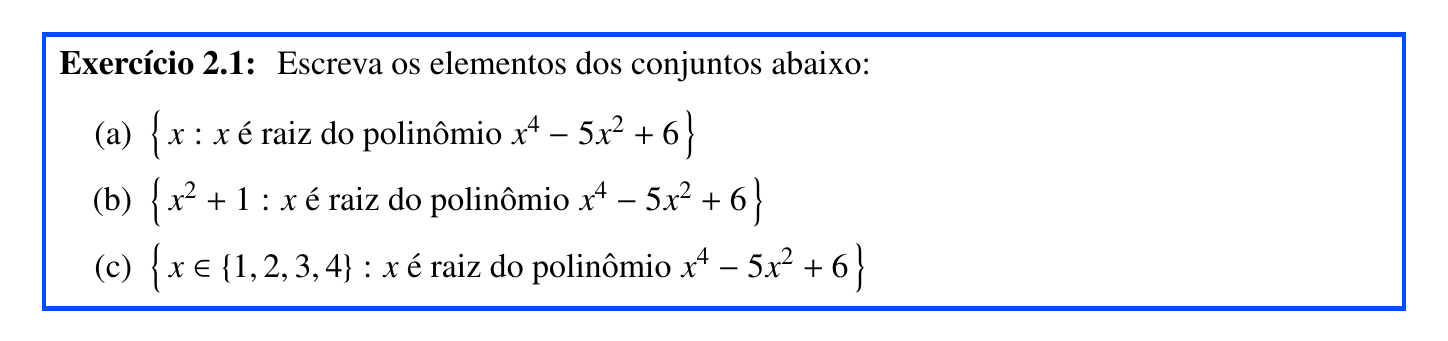
\includegraphics{images/ex-02.01.png}

\begin{tcolorbox}[enhanced jigsaw, coltitle=black, opacitybacktitle=0.6, toptitle=1mm, bottomtitle=1mm, colframe=quarto-callout-note-color-frame, leftrule=.75mm, colback=white, breakable, title={Resposta (a)}, titlerule=0mm, opacityback=0, toprule=.15mm, left=2mm, colbacktitle=quarto-callout-note-color!10!white, arc=.35mm, rightrule=.15mm, bottomrule=.15mm]

Precisamos usar algum método para resolver a equação

\[
x^4 - 5x^2 + 6 = 0
\]

Uma maneira: se fizermos $y = x^2$, a equação fica

\[
y^2 - 5y + 6 = 0
\]

que tem raízes $y = 2$ e $y = 3$.

Daí, resolvendo $2 = x^2$, temos $x = \pm\sqrt2$.

E resolvendo $3 = x^2$, temos $x = \pm\sqrt3$.

Escrevendo o conjunto como uma enumeração dos elementos:

\[
\left\{ -\sqrt3, -\sqrt2, \sqrt2, \sqrt3 \right\}
\]

\end{tcolorbox}

\begin{tcolorbox}[enhanced jigsaw, coltitle=black, opacitybacktitle=0.6, toptitle=1mm, bottomtitle=1mm, colframe=quarto-callout-note-color-frame, leftrule=.75mm, colback=white, breakable, title={Resposta (b)}, titlerule=0mm, opacityback=0, toprule=.15mm, left=2mm, colbacktitle=quarto-callout-note-color!10!white, arc=.35mm, rightrule=.15mm, bottomrule=.15mm]

Preste atenção: agora, não queremos as raízes, mas sim os valores de
$x^2 + 1$, onde $x$ assume os valores das raízes.

O conjunto poderia ser escrito como

\[
\left\{ x^2 + 1 : x \in \{ -\sqrt3, -\sqrt2, \sqrt2, \sqrt3 \} \right\}
\]

Calculando os valores de $x^2 + 1$, temos:

\begin{longtable*}{rr}
\toprule
\(x\) & \(x^2 + 1\) \\ 
\midrule\addlinespace[2.5pt]
\(-\sqrt{3}\) & \(4\) \\ 
\(-\sqrt{2}\) & \(3\) \\ 
\(\sqrt{2}\) & \(3\) \\ 
\(\sqrt{3}\) & \(4\) \\ 
\bottomrule
\end{longtable*}

Na tabela acima, há elementos repetidos, mas isto não pode acontecer em
um conjunto. Então, a resposta é

\[
\left\{ 3, 4 \right\}
\]

\subsubsection*{Em SETLX}\label{em-setlx}
\addcontentsline{toc}{subsubsection}{Em SETLX}

\begin{Shaded}
\begin{Highlighting}[]
\NormalTok{A := \{ {-}}\KeywordTok{sqrt}\NormalTok{(}\DecValTok{3}\NormalTok{), {-}}\KeywordTok{sqrt}\NormalTok{(}\DecValTok{2}\NormalTok{), }\KeywordTok{sqrt}\NormalTok{(}\DecValTok{3}\NormalTok{), }\KeywordTok{sqrt}\NormalTok{(}\DecValTok{2}\NormalTok{) \};}
\NormalTok{B := \{ x**}\DecValTok{2}\NormalTok{ + }\DecValTok{1}\NormalTok{ : x }\KeywordTok{in}\NormalTok{ A \};}
\KeywordTok{print}\NormalTok{(}\StringTok{"B = "}\NormalTok{, B);}

\CommentTok{// Como SETLX usou ponto flutuante, houve erro.}
\CommentTok{// Vamos arredondar:}
\KeywordTok{print}\NormalTok{( }\StringTok{"B = "}\NormalTok{, \{ }\KeywordTok{round}\NormalTok{(x) : x }\KeywordTok{in}\NormalTok{ B \} );}
\end{Highlighting}
\end{Shaded}

\begin{verbatim}
B = {3.0000000000000004, 3.9999999999999996}
B = {3, 4}
\end{verbatim}

\end{tcolorbox}

\bookmarksetup{startatroot}

\chapter*{Referências}\label{referuxeancias}
\addcontentsline{toc}{chapter}{Referências}

\markboth{Referências}{Referências}

\phantomsection\label{refs}
\begin{CSLReferences}{1}{0}
\bibitem[\citeproctext]{ref-anamaria23:_elemen_matem_discr_comput}
Anamaria Gomide, Jorge Stolfi. 2023. \emph{Elementos de Matemática
Discreta para Computação}.
\url{https://www.ic.unicamp.br/~stolfi/fmc-book/2022-08-24-js/livro.pdf}.

\end{CSLReferences}



\end{document}
